\begin{frame}
    \Huge
    \misc{
        Primera aproximación a la solución:\\
        Búsqueda de los parámetros por diferenciales
    }
\end{frame}

\begin{frame}
    \Huge
    \misc{
        \begin{equation*}
            RD=\left(\frac{Model - measurement}{measurement}\right)*100
        \end{equation*}
    }
\end{frame}

\begin{frame}
    \misc{
        \begin{figure}[H]
            \centering
            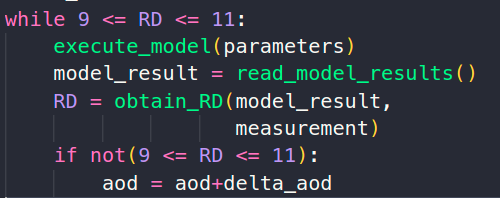
\includegraphics[width=14cm]{pseudo_code_1}
        \end{figure}
    }
\end{frame}

\begin{frame}
    \Huge
    \misc{
        Segunda aproximación a la solución:\\
        Búsqueda de los parámetros por medio del algoritmo de búsqueda binaria
    }
\end{frame}

\begin{frame}
    \misc{
        \begin{figure}[H]
            \centering
            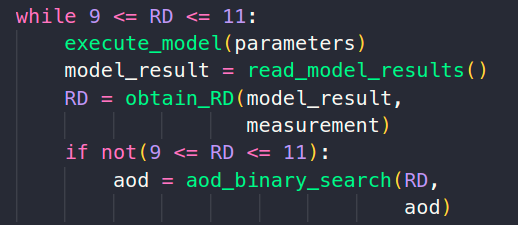
\includegraphics[width=12cm]{pseudo_code_2}
        \end{figure}
    }
\end{frame}

\begin{frame}
    \vspace{-1cm}
    \misc{
        \begin{figure}[H]
            \centering
            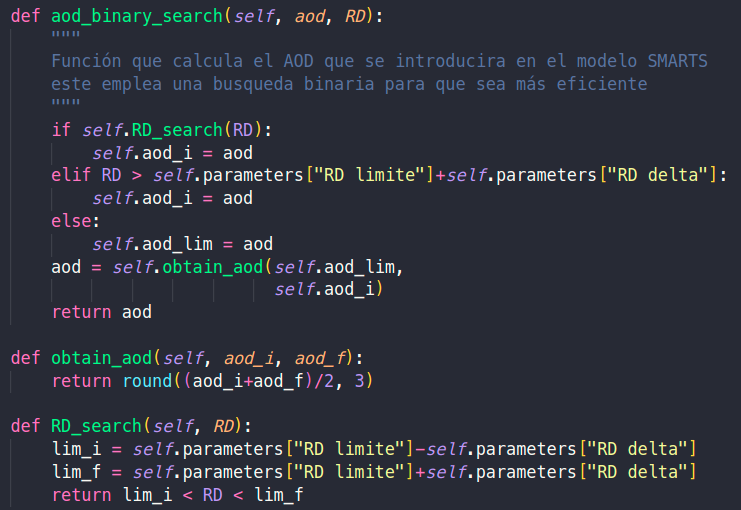
\includegraphics[width=11cm]{binary_search}
        \end{figure}
    }
\end{frame}

\begin{frame}
    \vspace{-1cm}
    \misc{
        \begin{minipage}{0.4\paperwidth}
            \begin{figure}[H]
                \centering
                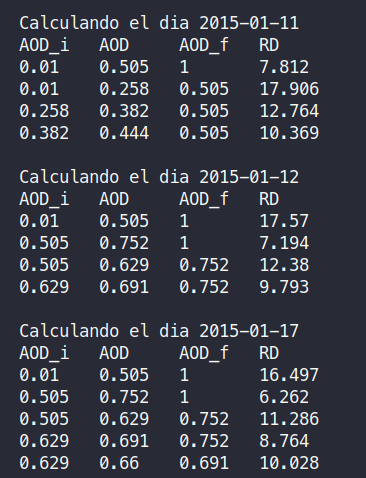
\includegraphics[height=7cm,width=5.5cm]{search_run}
            \end{figure}
        \end{minipage}
        \begin{minipage}{0.4\paperwidth}
            \begin{figure}[H]
                \centering
                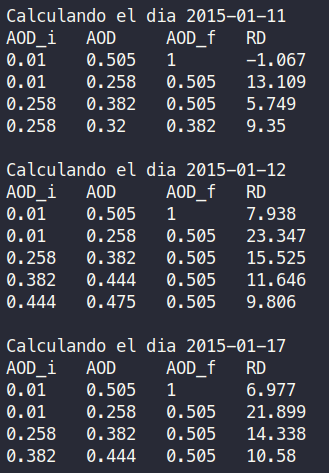
\includegraphics[height=7cm,width=5.5cm]{search_run_2}
            \end{figure}
        \end{minipage}
    }
\end{frame}

\begin{frame}
    \begin{figure}[H]
        \renewcommand{\yourowntexcol}{black}
        \centering
        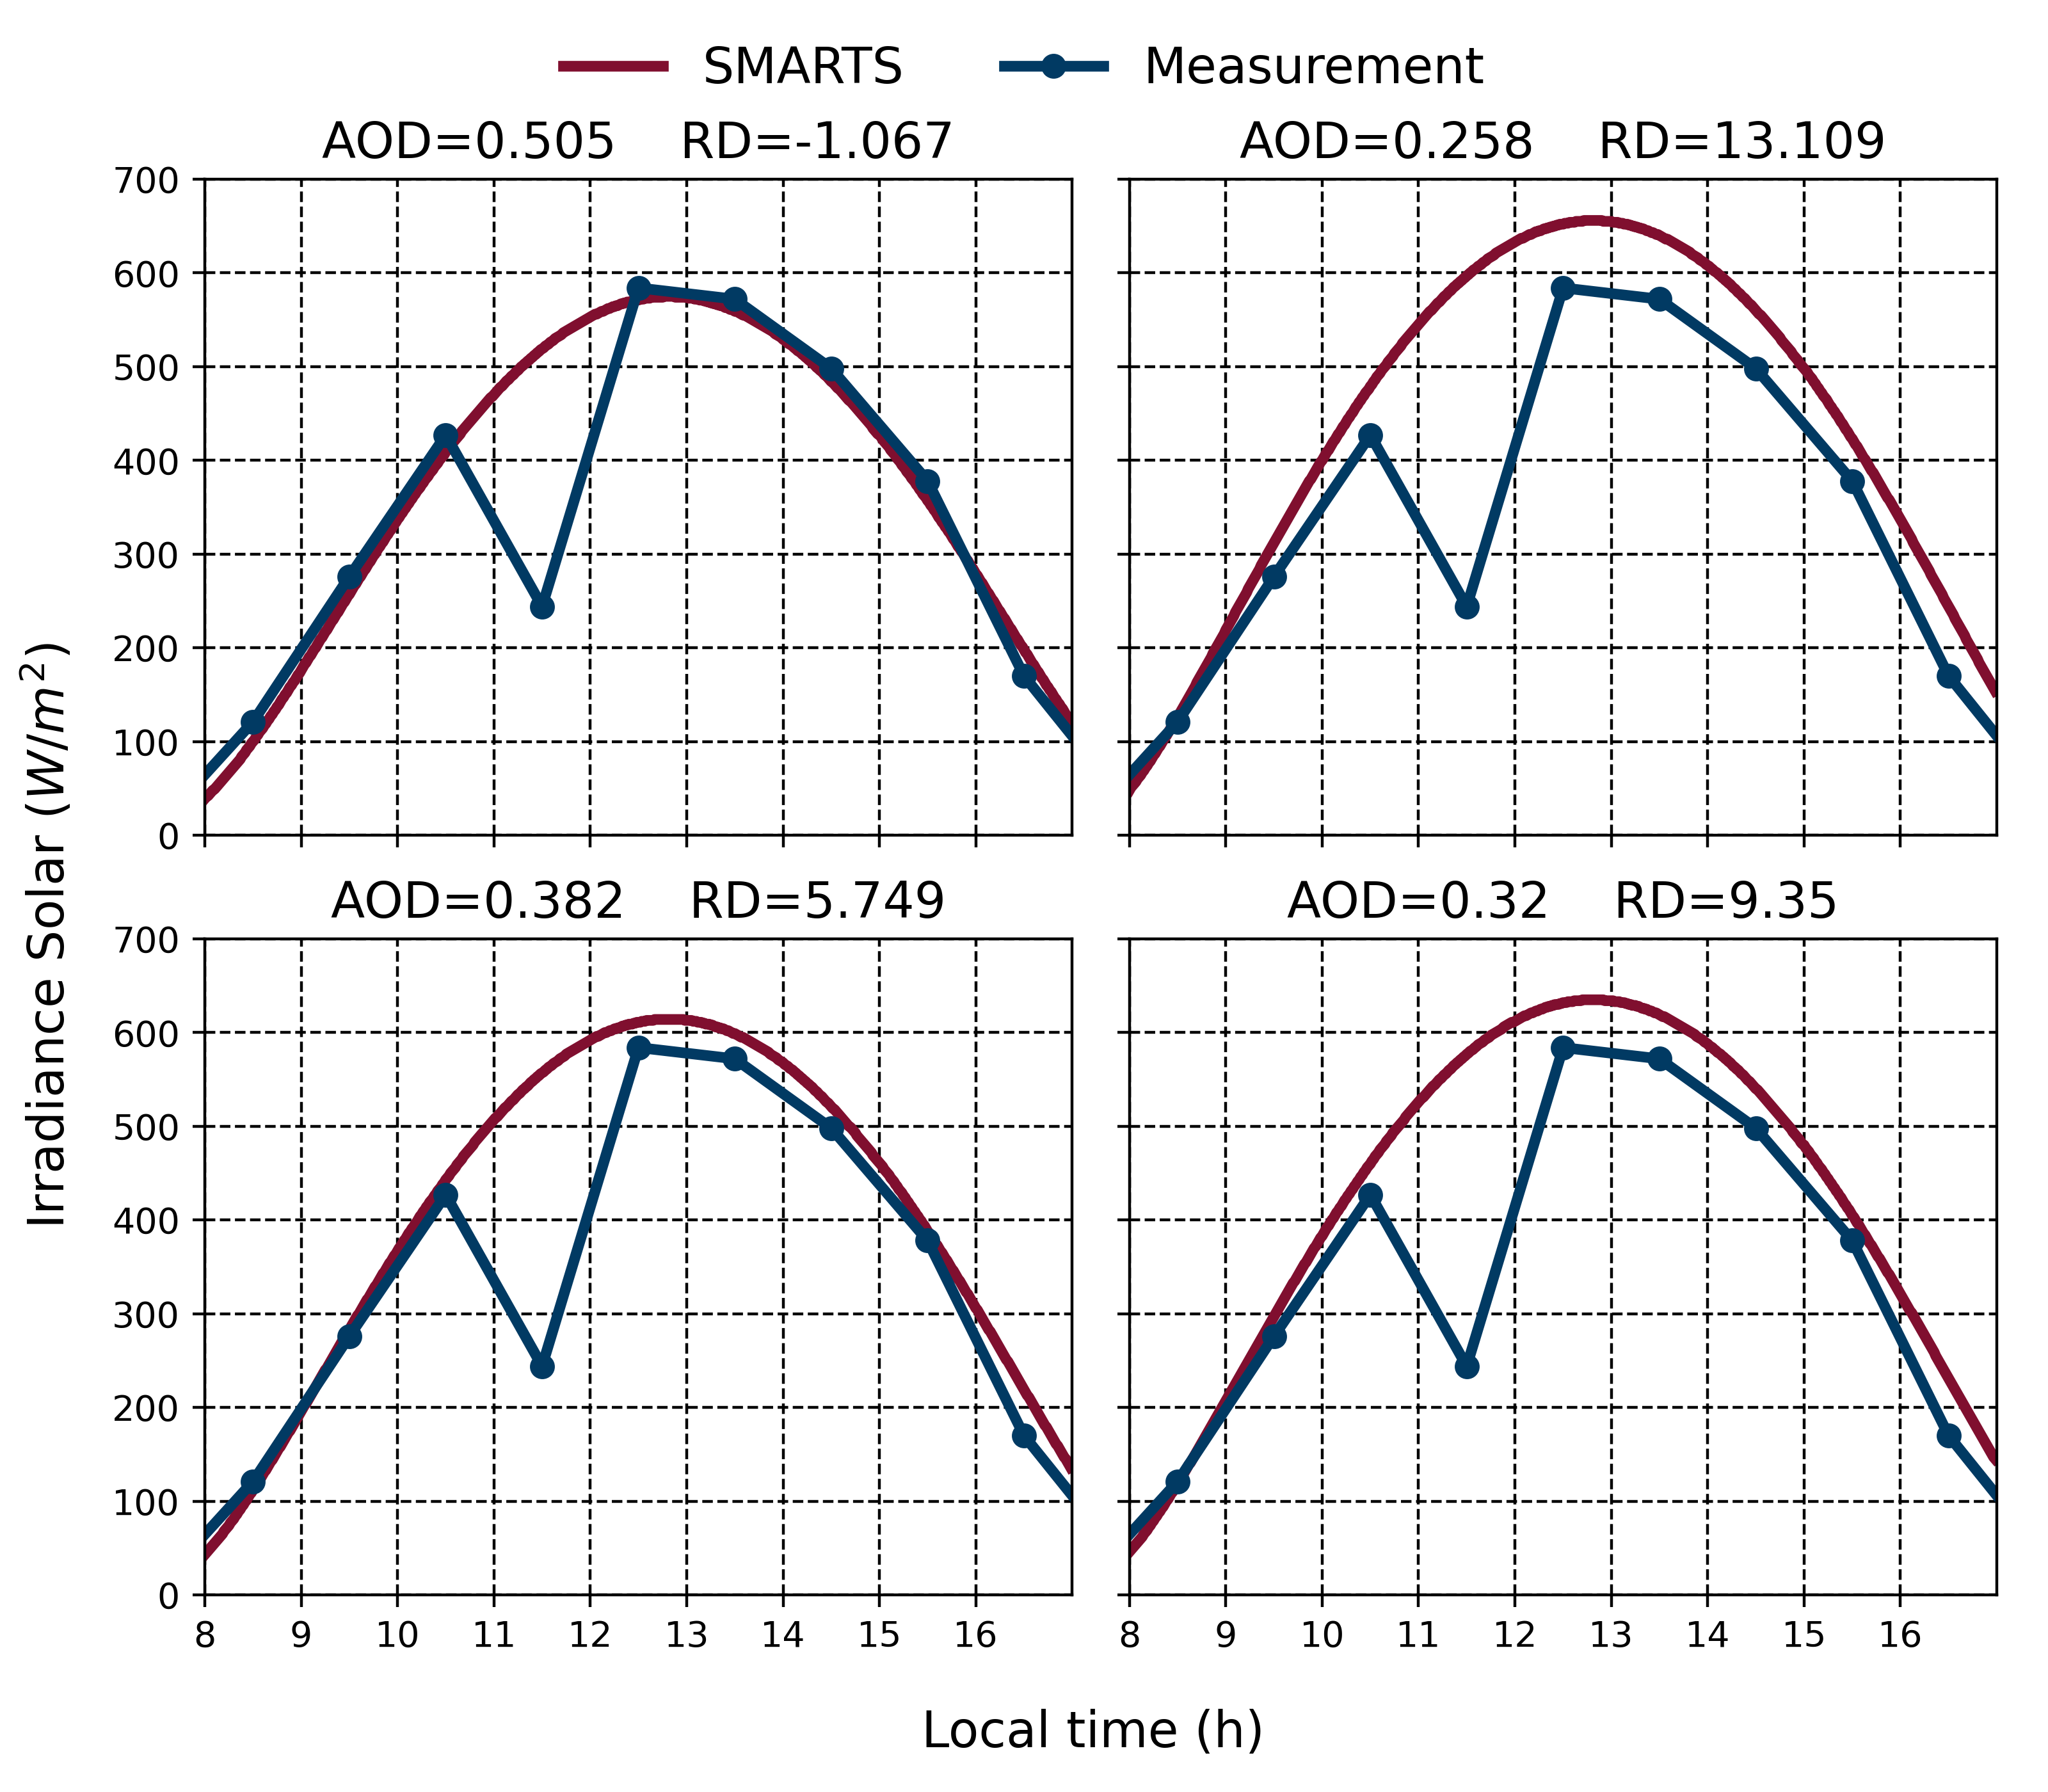
\includegraphics[width=0.7\paperwidth,height=0.85\paperheight]{Different_RD_values.png}
        \small
        \caption{Resultados del Modelo SMARTS haciendo uso de la búsqueda binaria.}
    \end{figure}
\end{frame}